\documentclass{article}
\usepackage[french]{babel}
\usepackage[T1]{fontenc}
\usepackage[utf8]{inputenc}
\usepackage{graphicx} % Required for inserting images
\usepackage{listingsutf8}
\usepackage{amsfonts}
\lstset{%
    inputencoding=utf8, 
    literate=
        {é}{{\'e}}{1}%
        {è}{{\`e}}{1}%
        {à}{{\`a}}{1}%
        {â}{{\^a}}{1}%
        {ç}{{\c{c}}}{1}%
        {œ}{{\oe}}{1}%
        {ù}{{\`u}}{1}%
        {É}{{\'E}}{1}%
        {È}{{\`E}}{1}%
        {À}{{\`A}}{1}%
        {Ç}{{\c{C}}}{1}%
        {Œ}{{\OE}}{1}%
        {Ê}{{\^E}}{1}%
        {ê}{{\^e}}{1}%
        {î}{{\^i}}{1}%
        {ï}{{\"i}}{1}%
        {ô}{{\^o}}{1}%
        {û}{{\^u}}{1}%
}
\usepackage{fullpage}
\usepackage{setspace}
\usepackage{todonotes}
\usepackage{amsthm}

\newtheoremstyle{exostyle}% style name
{10pt}% above space
{10pt}% below space
{}% body font
{}% indent amount
{\scshape\bfseries\large}% head font
{\hfill\vspace{5pt}\newline}% post head punctuation
{0pt}% Space after theorem head
{\hfill\thmname{#1}\thmnumber{ #2} -- \thmnote{ #3}}% head spec

\newtheoremstyle{partiestyle}% style name
{1em}% above space
{1em}% below space
{}% body font
{}% indent amount
{\bfseries}% head font
{\vspace{.5em}\newline}% post head punctuation
{0em}% Space after theorem head
{\thmnumber{#2} \thmnote{ #3}}% head spec

\newtheoremstyle{questionstyle}% style name
{.5em}% above space
{.5em}% below space
{}% body font
{}% indent amount
{\bfseries}% head font
{}% post head punctuation
{0em}% Space after theorem head
{Question \thmnumber{#2 }}% head spec

\theoremstyle{exostyle}
\newtheorem{exo}{Exercice}

\theoremstyle{partiestyle}
\newtheorem{partie}{}[exo]

\theoremstyle{questionstyle}
\newtheorem{question}{Question}[exo]
\newtheorem{questionpartie}{Question}[partie]

\title{Examen Terminal UE Programmation et Algorithmes}
\author{L1 MPCI}
\date{29 mai 2024 - Durée: 3h}

\begin{document}

\maketitle

\begin{center}
{\em\bf Lorsque l'on vous demande d'écrire de décrire ou de donner un algorithme cela signifiera toujours en donner un pseudo-code, justifier de son exactitude et de sa complexité}

~\\

{\em On rappelle qu'aucun document, ni équipement électrique ou électronique n'est autorisé. }
\end{center}


\vspace*{1cm}
Les exercices :
\begin{itemize}
\item sont au nombre de 3;
\item valent chacun 7 points (donc optimisez votre temps);
\item sont de difficulté équivalente;
\item sont indépendants;
\item leur début est plus facile que leur fin (qui vaudra donc plus de point).
\end{itemize}

\paragraph{}{\sc Rendez des copies séparées pour chaque exercice, ceci vous permettra de reprendre les exercices au cours de l'examen sans perdre le correcteur.}
\vspace*{1cm}

\clearpage

\begin{exo}[Champ de mines]
    Un champ de mines est représenté par une grille $M$ de $n\times n$ cases ($n$ lignes et $n$ colonnes) telle que $M[l][c]$ représente la probabilité de survie 
 d'une personne sur la case $(l, c)$ qui se trouve à la ligne $l$ et à la colonne $c$ (la probabilité d'existence d'une mine à la case $(l, c)$ vaut $1-M[l][c]$). On supposera qu'il n'y a jamais de mines en $(0,0)$ (la position initiale) et en $(n-1, n-1)$ (la sortie du champ de mines). La figure~\ref{champ} montre un champ de mines de taille $n=5$.

    \begin{figure}[h]
        \begin{center}
        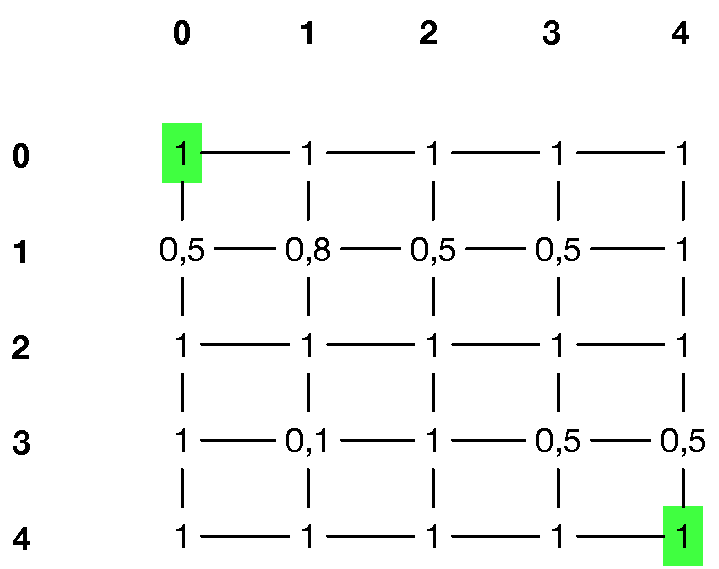
\includegraphics[scale=.5]{champ_mines}
        \end{center}
        \caption{Un champ de mines de taille 5\label{champ}}
    \end{figure}
    \paragraph{}Le but de l'exercice est de trouver un chemin $P = p_0\dots p_k$ allant de $p_0 = (0, 0)$ à $p_k = (n-1, n-1)$ permettant de sortir du champ de mines en maximisant ses chances de survie. 

    \paragraph{}Les contraintes de déplacement sont :

    \begin{itemize}
        \item on doit se déplacer à chaque étape,
        \item on ne peut se déplacer que d'une case à chaque étape,
        \item on ne peut se déplacer que horizontalement ou verticalement : si $p_i = (l_i, c_i)$ et $p_{i+1} = (l_{i+1}, c_{i+1})$, alors $\vert l_{i}-l_{i+1}\vert +\vert c_{i}-c_{i+1}\vert = 1$ pour tout $0\leq i < k$.

    \end{itemize}

\paragraph{} La figure~\ref{champ_chemin} montre un chemin de $k=8$ déplacements dont la probabilité d'arriver sain et sauf est de $\Pi_{0\leq i < k}M[l_i][c_i] = 0.5\times 0.1\times 0.5=2.5\%$.
    \begin{figure}[h]
        \begin{center}
        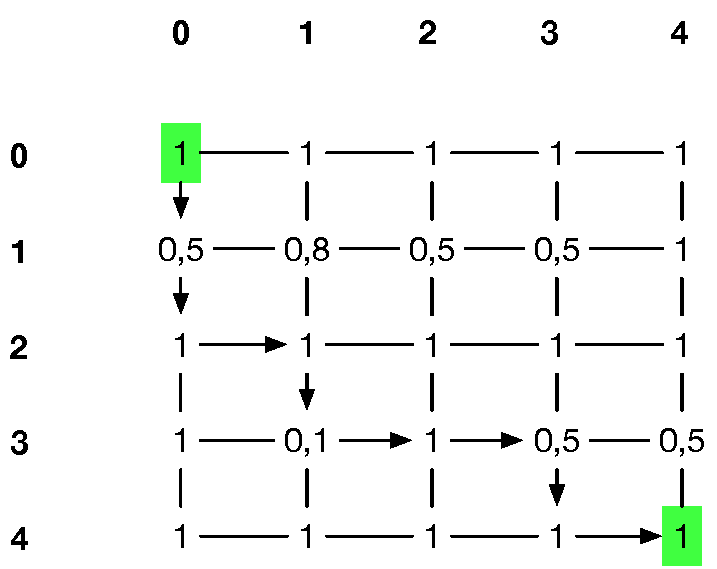
\includegraphics[scale=.5]{champ_mines_chemin}
        \end{center}
        \caption{Chemin $(0, 0)-(1, 0)-(2, 0)-(2, 1)-(3, 1)-(3, 2)-(3, 3)-(4, 3)-(4, 4)$\label{champ_chemin}}
    \end{figure}

    \begin{partie}[Exemple]
        \begin{questionpartie}
            Montrer sur l'exemple de la figure~\ref{champ_chemin} qu'il existe un chemin permettant d'atteindre la sortie du champ de mines avec une probabilité de 1.
        \end{questionpartie}
        \begin{questionpartie}
            Montrer sur l'exemple de la figure~\ref{champ_chemin} que si l'on ne peut pas revenir en arrière (à chaque déplacement soit la ligne soit la colonne augmente strictement), la probabilité de succès maximale n'est plus que de 80\%.
        \end{questionpartie}
    \end{partie}
    \begin{partie}[Validation des chemins]

        Un chemin est dit {\it valide} s'il respecte les contraintes de déplacement (on se déplace d'une ligne ou d'une colonne à chaque fois, en avant ou en arrière), commence au départ du champ et se termine à sa sortie.
        \begin{questionpartie}
     Montrer que l'on peut supposer sans perte de généralité qu'un chemin ne repasse jamais deux fois par la même case. Quelles sont les longueurs minimales et maximales d'un chemin permettant de sortir du champ de mines ?
        \end{questionpartie}
        \begin{questionpartie}
            Proposez un algorithme dont vous donnerez les paramètres, le code et la complexité permettant savoir si un chemin passé en paramètre est valide ou non.
        \end{questionpartie}
        \begin{questionpartie}
            Proposez un algorithme dont vous donnerez les paramètres, le code et la complexité permettant de connaître la probabilité de survie d'un chemin passé en paramètre respectant les contraintes de déplacement.
        \end{questionpartie}
    \end{partie}
    \begin{partie}[On avance]
        On rajoute une contrainte de déplacement supplémentaire : on ne peut pas reculer. C'est à dire que si $p_i = (l_i, c_i)$ et $p_{i+1} = (l_{i+1}, c_{i+1})$, alors $l_{i}\leq l_{i+1}$ et $c_{i} \leq c_{i+1}$ pour tout $0\leq i < k$.

        \begin{questionpartie}
            Proposez un algorithme dont vous donnerez les paramètres, le code et la complexité permettant de savoir si un chemin passé en paramètre respecte les contraintes de déplacement.
        \end{questionpartie}
            
            \paragraph{}On note $S$ la matrice carrée à $n$ lignes telle que $S[l][c]$ soit la probabilité de survie maximale d'un chemin allant de $(0,0)$ à $(l, c)$. 
        \begin{questionpartie}
            En utilisant le principe de la programmation dynamique que vous explicitez, donnez une équation permettant de calculer $S[l][c]$ à partir des éléments $S[l'][c']$ avec $0 \leq l' < l < n$ et $0 \leq c' < c < n$.
        \end{questionpartie}
        \begin{questionpartie}
            En déduire un algorithme dont vous expliciterez les paramètres, le code et la complexité permettant de trouver $S[n-1][n-1]$.
        \end{questionpartie}
        \begin{questionpartie}
            Explicitez en quelques lignes comment faire pour retrouver un chemin maximisant la probabilité de sortie du champ de mines en connaissant la matrice $S$.
        \end{questionpartie}
    \end{partie}
    \begin{partie}[Cas général]
        La contrainte supplémentaire ajoutée dans la partie précédente est supprimée : on peut atteindre chaque case $(l, c)$ du champ par ses 4 voisins ($(l-1, c)$, $(l+1, c)$, $(l, c-1)$ et $(l, c+1)$).
        \begin{questionpartie}
      Montrez que l'on ne peut plus utiliser l'algorithme de la partie précédente pour résoudre le problème. 
        \end{questionpartie}

            \paragraph{}On note $S$ la matrice tri-dimensionnelle carrée à $n$ lignes telle que $S[k][l][c]$ soit la probabilité de survie maximale d'un chemin d'au plus $k$ déplacements allant de $(0,0)$ à $(l, c)$. 
        \begin{questionpartie}
            Quelles sont les valeurs de $S[0][l][c]$ pour $0\leq l, c < n$ ?
        \end{questionpartie}
        \begin{questionpartie}
       Quelle case de la matrice tri-dimensionnelle $S$ correspond à la probabilité maximale de survie pour sortir du champ de mines ?
        \end{questionpartie}
        \begin{questionpartie}
            En utilisant le principe de la programmation dynamique, donnez une équation permettant de calculer $S[k][l][c]$ à partir des éléments $S[k-1][l'][c']$ avec $0 \leq l', l < n$ et $0 \leq c', c < n$.
        \end{questionpartie}
        \begin{questionpartie}
            En déduire un algorithme dont vous expliciterez les paramètres, le code et la complexité permettant de trouver la probabilité maximale de sortie d'un champ de mines.
        \end{questionpartie}
        \begin{questionpartie}
Donner un algorithme dont vous expliciterez les paramètres, le code et la complexité permettant de renvoyer un chemin de probabilité maximale de sortie d’un champ de mines        \end{questionpartie}

    \end{partie}
\end{exo}

\clearpage
\begin{exo}[Fichiers et dossiers d'un disque dur]

On souhaite créer des classes pour manipuler les fichiers et dossiers présents sur un disque dur. 

\paragraph{}On rappelle qu'un disque dur est organisé selon une arborescence et contient des éléments pouvant être des {\it dossiers} ou des {\it fichiers}. L'élément de départ, nommé racine, est un dossier et par convention s'appelle "/". Les dossiers sont des éléments permettant de stocker d'autres éléments (dossiers ou fichiers)  et les fichiers sont des éléments qui peuvent être lus (des textes ou des images par exemple) ou exécutés (le programme python par exemple).

La figure~\ref{fig-fichiers} montre un exemple de disque dur :

\begin{figure}[h]
\centering
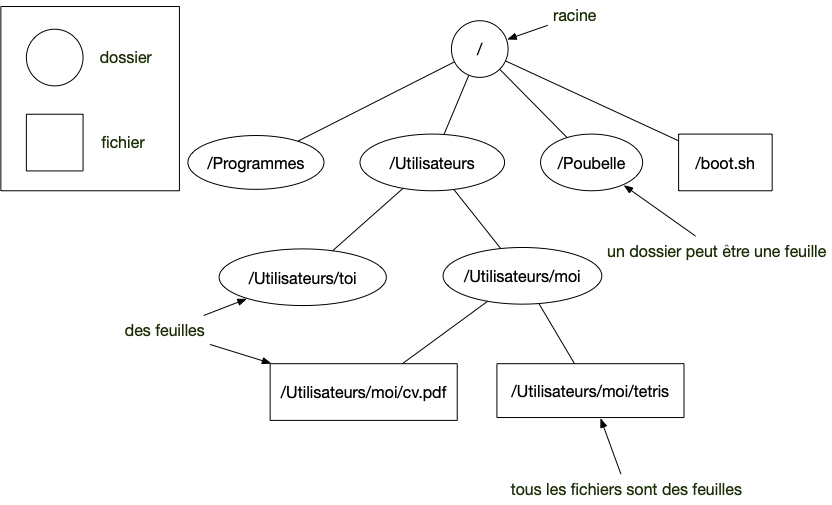
\includegraphics[scale=.5]{arborescence.png}
    
\caption{Les dossiers et fichiers d'un disque dur.\label{fig-fichiers}}

\end{figure}

On utilise souvent une métaphore familiale pour désigner les éléments de cette arborescence : les {\it enfants} d'un dossier sont les éléments qu'il contient (fichier ou dossier) et chaque élément différent de la racine contient un unique dossier {\it parent}. Par exemple pour l'arborescence de la figure~\ref{fig-fichiers} : les enfants de la racine sont les dossiers \verb`Programmes`, \verb`Utilisateurs` et \verb`Poubelle`, ainsi que le fichier \verb`boot.sh` ; le père du dossier \verb`moi` est le dossier \verb`Utilisateurs`.


\paragraph{}On supposera ici que le nom d'un fichier ou d'un dossier est uniquement composé de lettres de l'alphabet, des caractères \verb+"."+ et \verb+"_"+ ; sauf le dossier racine dont le nom est \verb`"/"`.

On peut représenter un endroit dans le disque dur par un {\it chemin} qui est une chaîne de caractères reprenant les noms des différents dossiers permettant d'aller de la racine à l'endroit voulu séparé par des "\verb`/`". Ainsi la chaîne \verb`"/Utilisateurs/toi"` correspond à l'élément de nom \verb`"toi"` et de chemin \verb`"/Utilisateurs/"` (le fichier est stocké dans le dossier de nom \verb`"Utilisateurs"` lui-même stocké dans la racine).


\begin{partie}[Modèle UML]
On veut dans cette partie faire une modélisation UML de cette organisation.

\begin{questionpartie}
\label{uml}
Proposez une modélisation UML des classes \verb`Fichier` et \verb`Dossier`. On doit pouvoir :

\begin{itemize}
    \item créer un fichier ou un dossier grâce à son nom et à son dossier parent (la racine sera créée avec un dossier parent valant \verb`None`).
    \item connaître le nom du fichier ou du dossier,
    \item connaître le chemin du dossier ou du fichier,
    \item connaître le dossier parent du fichier ou du dossier,
    \item connaître tous les éléments stockés dans un dossier,
    \item savoir si un fichier est un programme exécutable (comme le programme python) ou non (comme un fichier texte par exemple). Pour cela, un \verb`Fichier` doit avoir une méthode \verb`est_exécutable()`.

\end{itemize}

\end{questionpartie}
\begin{questionpartie}
En supposant que les classes \verb`Fichier` et \verb`Dossier` sont dans le fichier \verb`"disque_dur.py"`, écrivez le code permettant de créer l'exemple de la figure~\ref{fig-fichiers} (on ne demande pas d'écrire le code des classes ici, mais seulement de les utiliser, en supposant qu'elles existent).

\end{questionpartie}

\begin{questionpartie}
Certaines fonctionnalités sont identiques entre les classes \verb`Fichier` et \verb`Dossier`. Comment faire pour ne pas avoir à re-écrire plusieurs fois le même code ?\end{questionpartie}

\end{partie}
\begin{partie}[Code des classes]
\begin{questionpartie}
Écrivez le constructeur de la classe \verb`Dossier`.
\end{questionpartie}
\begin{questionpartie}
Écrivez la méthode permettant de connaître le chemin d'un \verb`Dossier` ou d'un \verb`Fichier` en utilisant les attributs et méthodes que vous avez décrits à la question~\ref{uml}. Par exemple, pour le fichier de nom \verb`"cv.pdf"` de la figure~\ref{fig-fichiers}, la méthode rendra la chaîne de caractères \verb`"/Utilisateurs/moi/cv.pdf"`.
\end{questionpartie}
\begin{questionpartie}
Donnez le code complet de la classe \verb`Fichier`. 
\end{questionpartie}

\end{partie}
\begin{partie}[Énumération]
\begin{questionpartie}
\label{algo-parcours}
Écrivez une fonction permettant d'afficher un à un le nom de chaque élément (\verb`Dossier` et \verb`Fichier`) d'une arborescence. Cette fonction prendra un \verb`Dossier` en paramètre et pourra être récursive.
\end{questionpartie}
\begin{questionpartie}
Explicitez la complexité de la fonction de la question précédente.
\end{questionpartie}
\begin{questionpartie}
Dans quel ordre sont parcourus les éléments de l'arborescence pour l'algorithme de la question~\ref{algo-parcours} ? Explicitez ce parcours sur l'exemple de la figure~\ref{fig-fichiers}.
\end{questionpartie}

\end{partie}
\end{exo}

\clearpage
\begin{exo}[Fenêtres bariolées]
 Soit $K$ un entier strictement positif et $s = s_0\dots s_{n-1}$ une liste de $n$ entiers telle que $\{s_i \vert 0\leq i < n \} = \{0, \dots, K-1\}$.
 Une {\it fenêtre bariolée de $s$} est une sous-liste $s[i:j+1] = s_i\dots s_j$, avec $0 \leq i \leq j < n$, contenant tous les entiers de $0$ à $K-1$ ($\{s_l \vert 0\leq i \leq l \leq j < n \} = \{0, \dots, K-1\}$). Notez que $K$ est définie pour la liste initiale, pas la sous liste. 

\begin{partie}[Sous-liste]

Soit \verb`tous(K, liste)` une fonction qui rend \verb`True` si la liste \verb`liste` contient tous les entiers entre 0 et K-1 (inclus).

\begin{questionpartie}
Proposez un algorithme qui implémente \verb`tous(K, liste)`. Vous expliciterez sa complexité et donnerez le nombre de cases mémoires utilisées. 
\end{questionpartie}
\begin{questionpartie}
Proposez un algorithme nommé \verb`ok_K(l)` prenant en paramètre une liste $l=l_0\dots l_{n-1}$ et rendant `True` s'il existe $K$ tel que $\{l_i \vert 0\leq i < n \} = \{0, \dots, K-1\}$. Vous utiliserez \verb`tous(K, liste)` pour créer cet algorithme. 
Vous expliciterez sa complexité. 

\end{questionpartie}

\begin{questionpartie}
    Soit \verb`suite` une liste telle que \verb`ok_K(suite) == True`. Donner le code et la complexité d'une fonction \verb`fenêtre(i, j, suite)` rendant \verb`True` si $\mbox{liste}[i:j+1]$ est une fenêtre bariolée de \verb`suite`.
\end{questionpartie}

\end{partie}

\begin{partie}[Glouton]
\begin{questionpartie}
Proposez un algorithme glouton dont vous donnerez les paramètres, le code et la complexité permettant de trouver une fenêtre bariolée $s[0:j+1]$ à partir d'une liste $s$ telle que \verb`tous(K, s) == True` telle que $s[0:j]$ ne soit pas bariolée.

Vous expliciterez pourquoi cet algorithme est glouton, pourquoi il trouve bien une fenêtre bariolée et pourquoi elle est minimale.
\end{questionpartie}

\begin{questionpartie}
Proposez un algorithme glouton prenant une suite $s$ et un entier $i^\star$ en paramètres et rendant l'entier $j$ le plus petit possible pour que  $s[i^\star:j+1]$ soit une fenêtre bariolée de $s$. Vous donnerez également la complexité de cet algorithme.

\end{questionpartie}
\begin{questionpartie}
En déduire un algorithme dont vous donnerez les paramètres, le code et la complexité pour déterminer la plus petite longueur d’une fenêtre bariolée d'une liste $s$ telle que \verb`tous(K, s) == True`.
\end{questionpartie}

\end{partie}

\begin{partie}[Optimal]

On cherche maintenant à trouver une fenêtre bariolée $s[i:j+1]$ de taille ($j+1-i$) minimum le plus rapidement possible.
\begin{questionpartie}
Montrez que la complexité du problème de la recherche d'une fenêtre bariolée à partir de $s$ et de $K$ ($K$ est donné et $s$ est telle que  $\{s_i \vert 0\leq i < n \} = \{0, \dots, K-1\}$) est au moins en $\mathcal{O}(n)$.
\end{questionpartie}

\begin{questionpartie}
Donnez une condition nécessaire et suffisante impliquant $s[i]$ pour que $s[i+1:j+1]$ soit bariolée si $s[i:j+1]$ l'est.
\end{questionpartie}

\begin{questionpartie}
En déduire un algorithme dont vous donnerez les paramètres et le code, de complexité $\mathcal{O}(n)$ et nécessitant $\mathcal{O}(K)$ cases mémoires pour résoudre le problème de trouver une fenêtre bariolée de taille minimum.
\end{questionpartie}

\end{partie}
\end{exo}
\end{document}